\documentclass[11pt]{scrartcl}
\usepackage[utf8]{inputenc}
\usepackage[sexy]{evanchen} 
\usepackage{graphicx}
\graphicspath{{8 Outsource K Math/Gambar/}}

\title{Lingkaran Sembilan Titik}
\author{Azzam and Akeyla}

\begin{document}

\maketitle

\section{Pendahuluan}
Lingkaran sembilan titik (\textit{Nine-point circle}) adalah lingkaran yang melewati sembilan titik yang cukup penting dari sembarang segitiga. Kesembilan titik tersebut adalah :
\begin{enumerate}
    \item Titik tengah ketiga sisi segitiga
    \item Proyeksi dari ketiga titik sudut segitiga ke sisi di hadapannya
    \item Titik tengah dari segmen garis yang menghubungkan titik sudut segitiga dengan titik tinggi segitiga.
\end{enumerate} 
\section{Dua Lemma yang Cukup Penting}
Sebelum membuktikan keberadaan lingkaran sembilan titik, terlebih dahulu di\medskip berikan dua lemma yang akan berguna.
\newline
\begin{theorem}
\textbf{Lemma 1.} Diberikan segitiga $ABC$ dengan $H$ sebagai titik tinggi. Maka pen\smallskip cerminan titik $H$ terhadap sisi $BC$ berada di lingkaran luar segitiga $ABC$.\newline

\end{theorem}

% \textbf{Bukti:}\\

\begin{figure}[h]
    \centering
    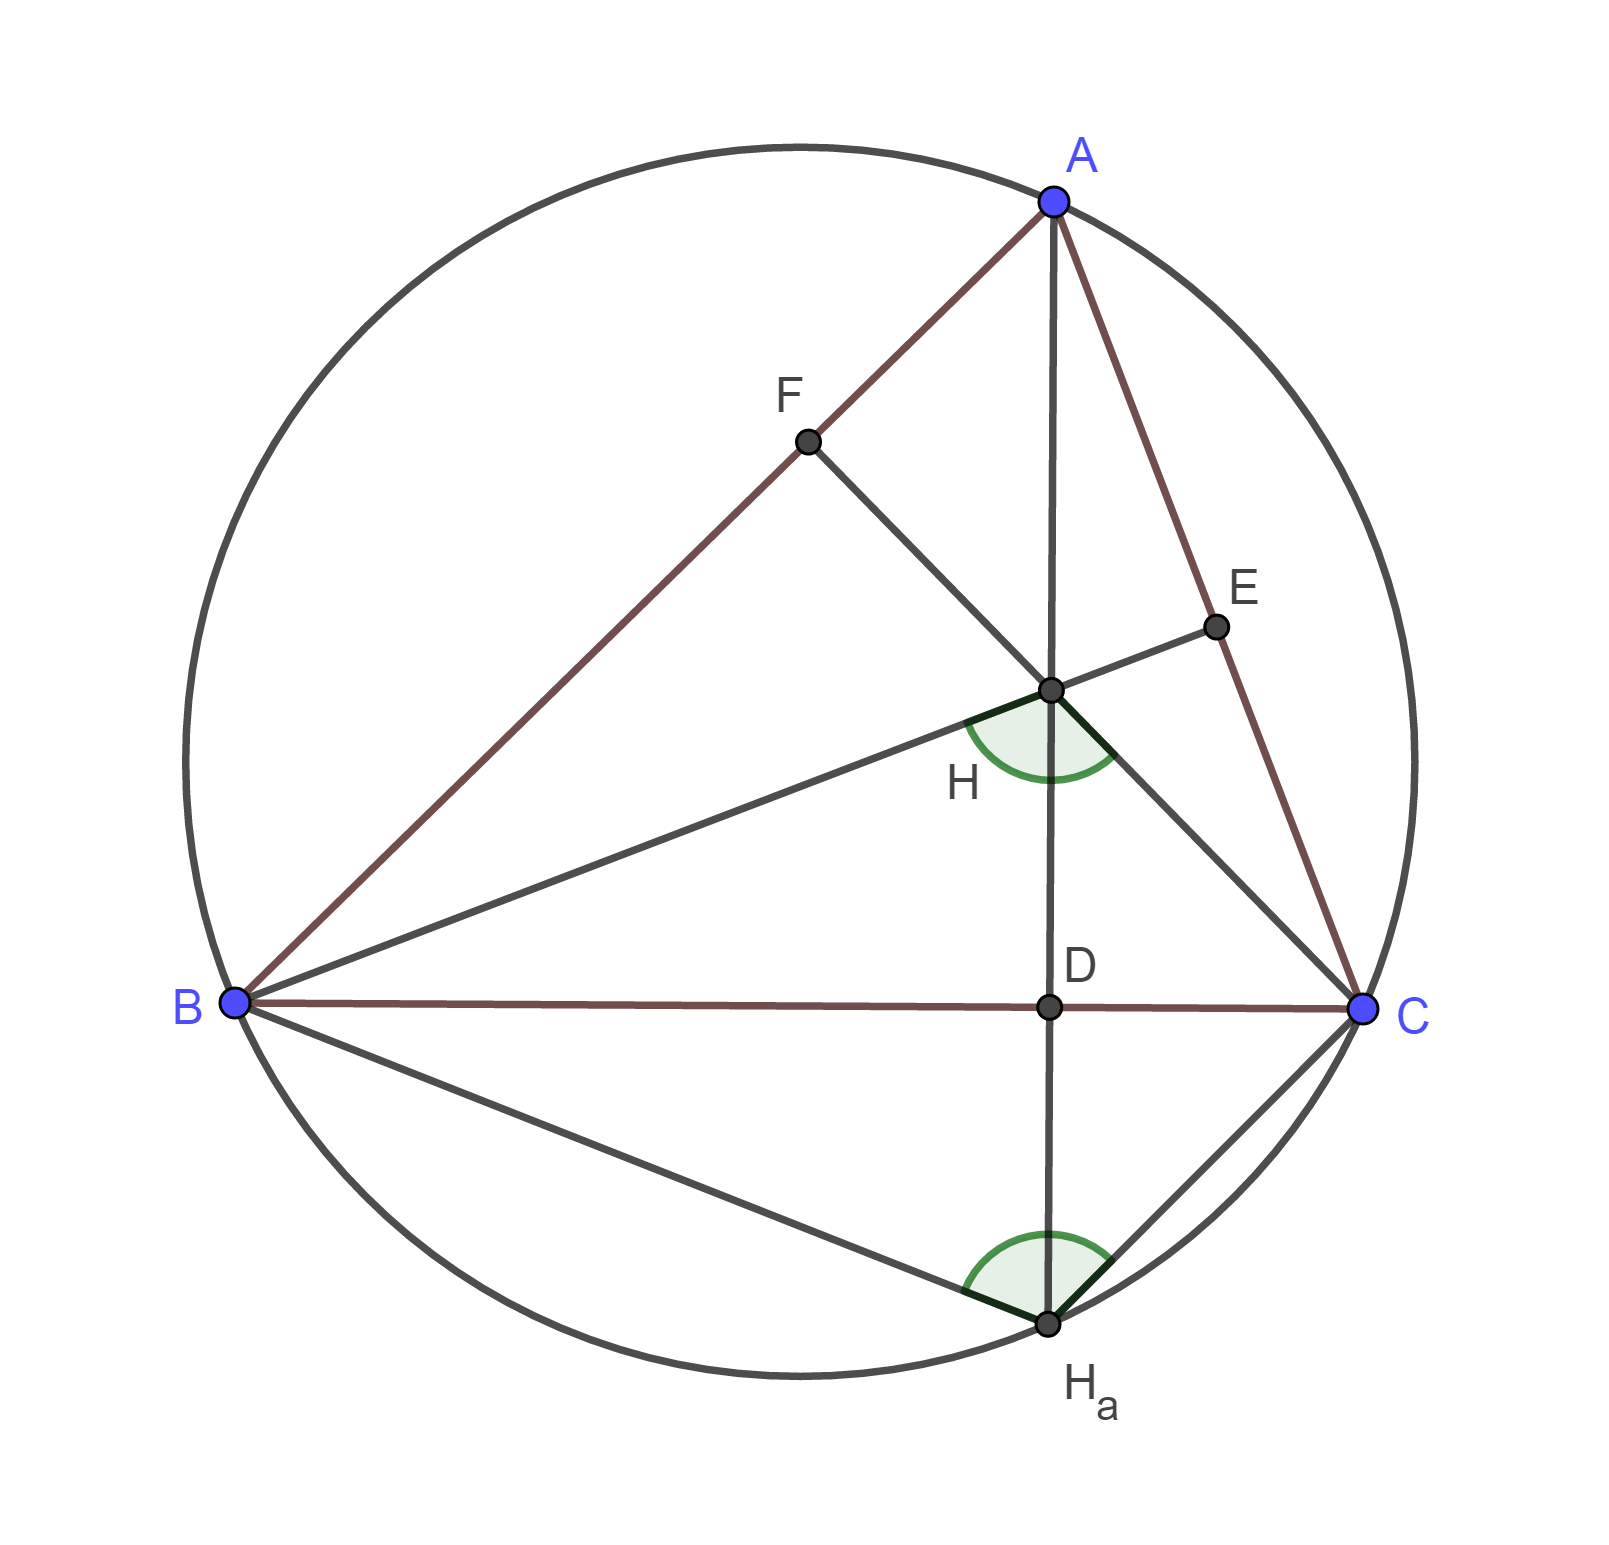
\includegraphics[width=6cm]{LEMMA1N9.png}
\end{figure}

% Kita akan tinjau bukti untuk kasus segitiga $ABC$ lancip. Untuk segitiga $ABC$ tumpul dan siku-siku dapat dibuktikan dengan cara yang serupa.\\
% Misalkan $D,E,F$ secara berurutan adalah proyeksi titik $A,B,C$ ke sisi di hadapannya dan $H_a$ adalah pencerminan titik $H$ terhadap sisi $BC$.\\
% Maka, $\angle{HEA} = \angle{HFA} = 90^\circ$.\\
% Karena $\angle{HEA} + \angle{HFA} = 180^\circ$, maka segiempat $HEAF$ siklik dan akibatnya, $$\angle{EHF} = 180^\circ - \angle{EAF} = 180^\circ - \angle{BAC}$$
% Karena $H_a$ adalah pencerminan titik $H$ terhadap garis $BC$ maka $$\angle{BH_aC} = \angle{BHC}$$
% Namun, $$\angle{BHC} = \angle{EHF} = 180^\circ - \angle{BAC}$$
% Maka, $$\angle{BH_aC} + \angle{BAC} = 180^\circ$$
% Sehingga segiempat $BH_aCA$ siklik dan akibatnya $H_a$ terletak di lingkaran luar \bigskip segitiga $ABC$.\\ 

\begin{theorem}
\textbf{Lemma 2.} Diberikan segitiga $ABC$ dengan $H$ titik tinggi dan $M$ titik tengah sisi $BC$. Maka pencerminan titik $H$ terhadap titik $M$ berada di lingkaran luar segitiga $ABC$.    
\end{theorem}
% \textbf{Bukti :}\\
\begin{figure}[h]
    \centering
    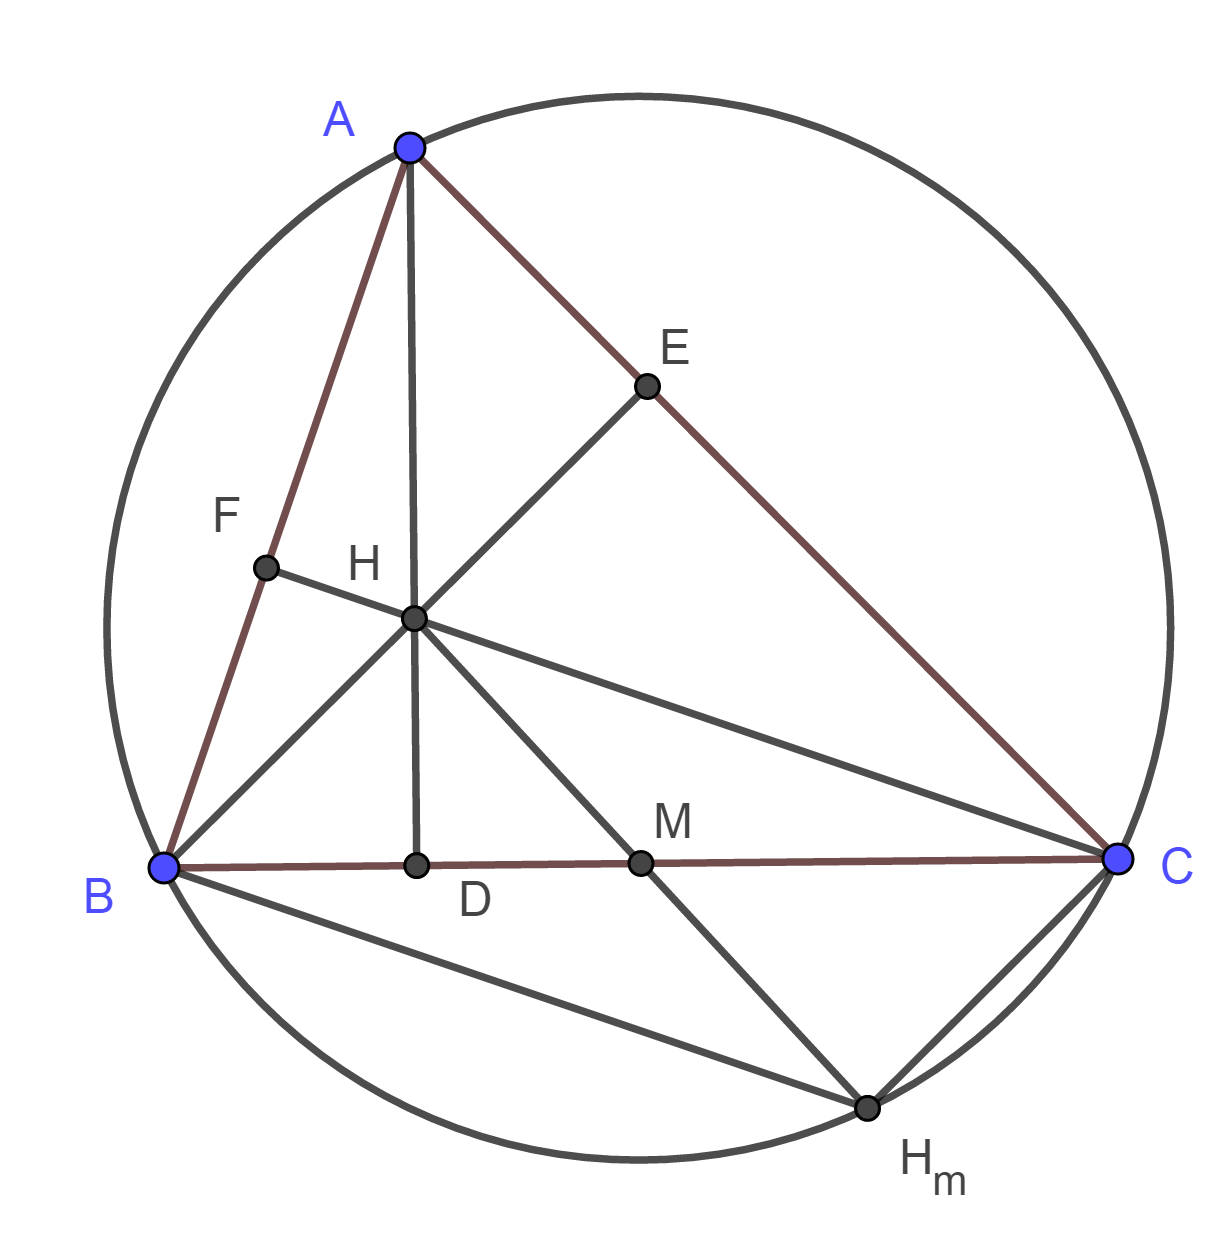
\includegraphics[width=6cm]{lemma2N9.png}
\end{figure}
% Kembali kita tinjau bukti untuk kasus segitiga $ABC$ lancip.\\
% Misalkan $H_m$ adalah hasil pencerminan titik $H$ terhadap titik $M$, maka perhatikan bahwa $M$ adalah titik tengah $BC$ sekaligus titik tengah $HH_m$. Akibatnya, $HCH_mB$ adalah jajargenjang.\\
% Maka, $$\angle{BH_mC} = \angle{BHC} = 180^\circ -\angle{BAC}$$
% Oleh karena itu, $ABH_mC$ adalah segiempat siklis dan $H_m$ terletak di lingkaran luar segitiga $ABC$.
\section{Diagram yang Lebih Lengkap}
Diberikan segitiga $ABC$ dengan $D,E$ dan $F$ berturut-turut adalah proyeksi titik $A,B$ dan $C$ ke sisi yang ada di hadapannya serta $H$ dan $O$ berturut-turut adalah titik tinggi dan titik pusat lingkaran luar $\Delta ABC$. Misalkan $M,N$ dan $P$ berturut-turut adalah titik tengah $BC,CA$ dan $AB$. Misalkan pula $H_a,H_b$ dan $H_c$ berturut-turut adalah pencerminan titik $H$ terhadap sisi $BC,CA$ dan $AC$ serta $H_m,H_n,H_p$ berturut-turut adalah pencerminan titik $H$ terhadap $M,N,P$.\\
Berdasarkan Lemma 1 dan Lemma 2, titik $H_a,H_b,H_c,H_m,H_n,H_p$ bersama dengan $A,B,C$ terletak di lingkaran luar segitiga $ABC$.
\begin{figure}[h]
    \centering
    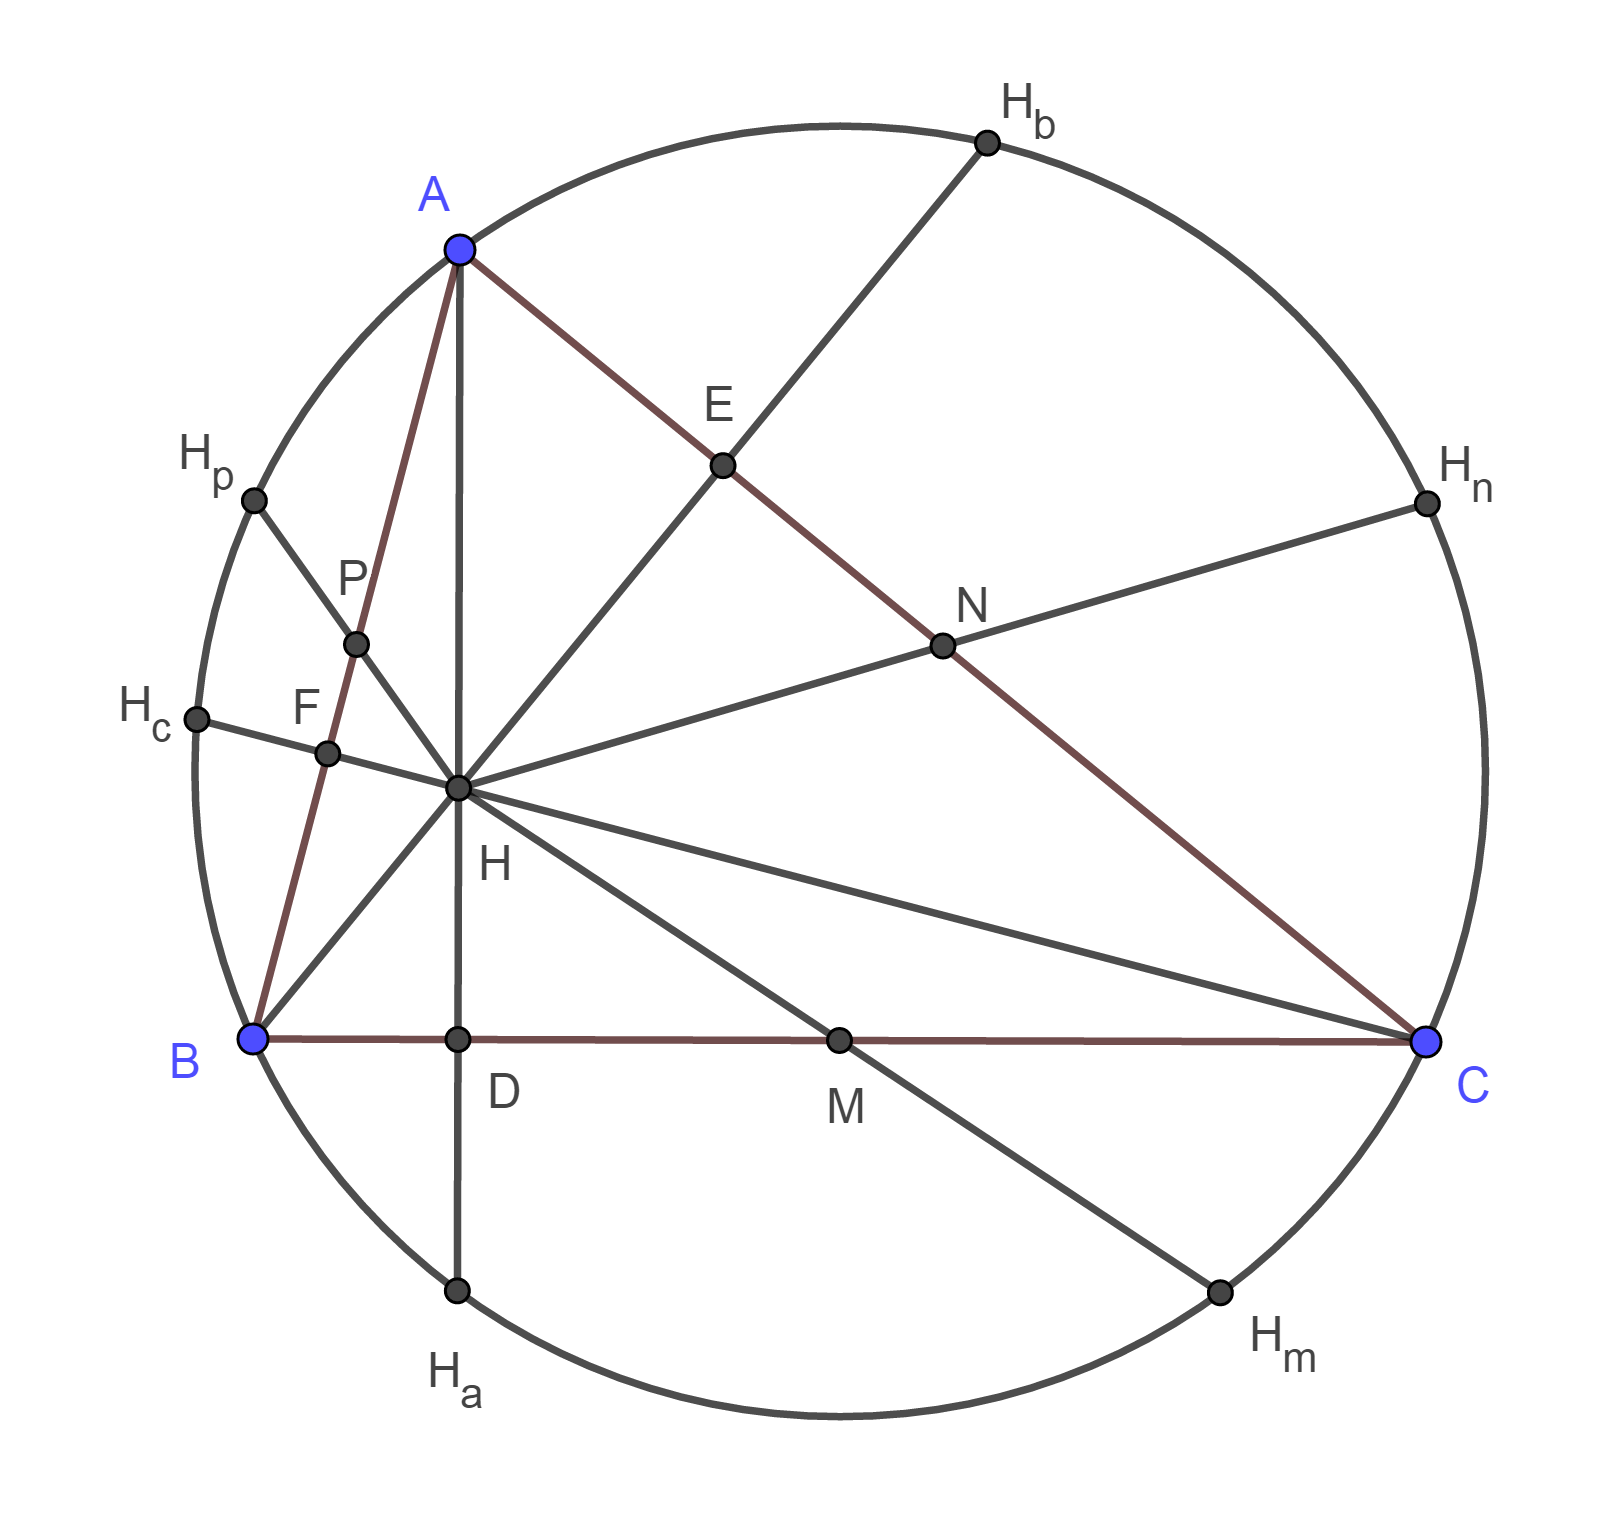
\includegraphics[width=6cm]{gg3.png}
\end{figure}
\\Tinjau homotethy $h$ dengan pusat $H$ dan skala $\frac{1}{2}$. Homotethy ini mengirim titik $H_a,H_b,H_c,H_m,H_n,H_p$ berturut-turut ke titik $D,E,F,M,N,P$ dan titik $A,B,C$ berturut-turut ke titik tengah $AH,BH,CH$, sebut saja $A_h,B_h$ dan $C_h$. Dan karena homotethy mempertahankan sifat siklik, maka kesembilan titik $D,E,F,M,N,P,A_h,B_h,C_h$ juga siklik. Sebut lingkaran yang memuat kesembilan titik ini sebagai $\omega_9$.
\begin{figure}
    \centering
    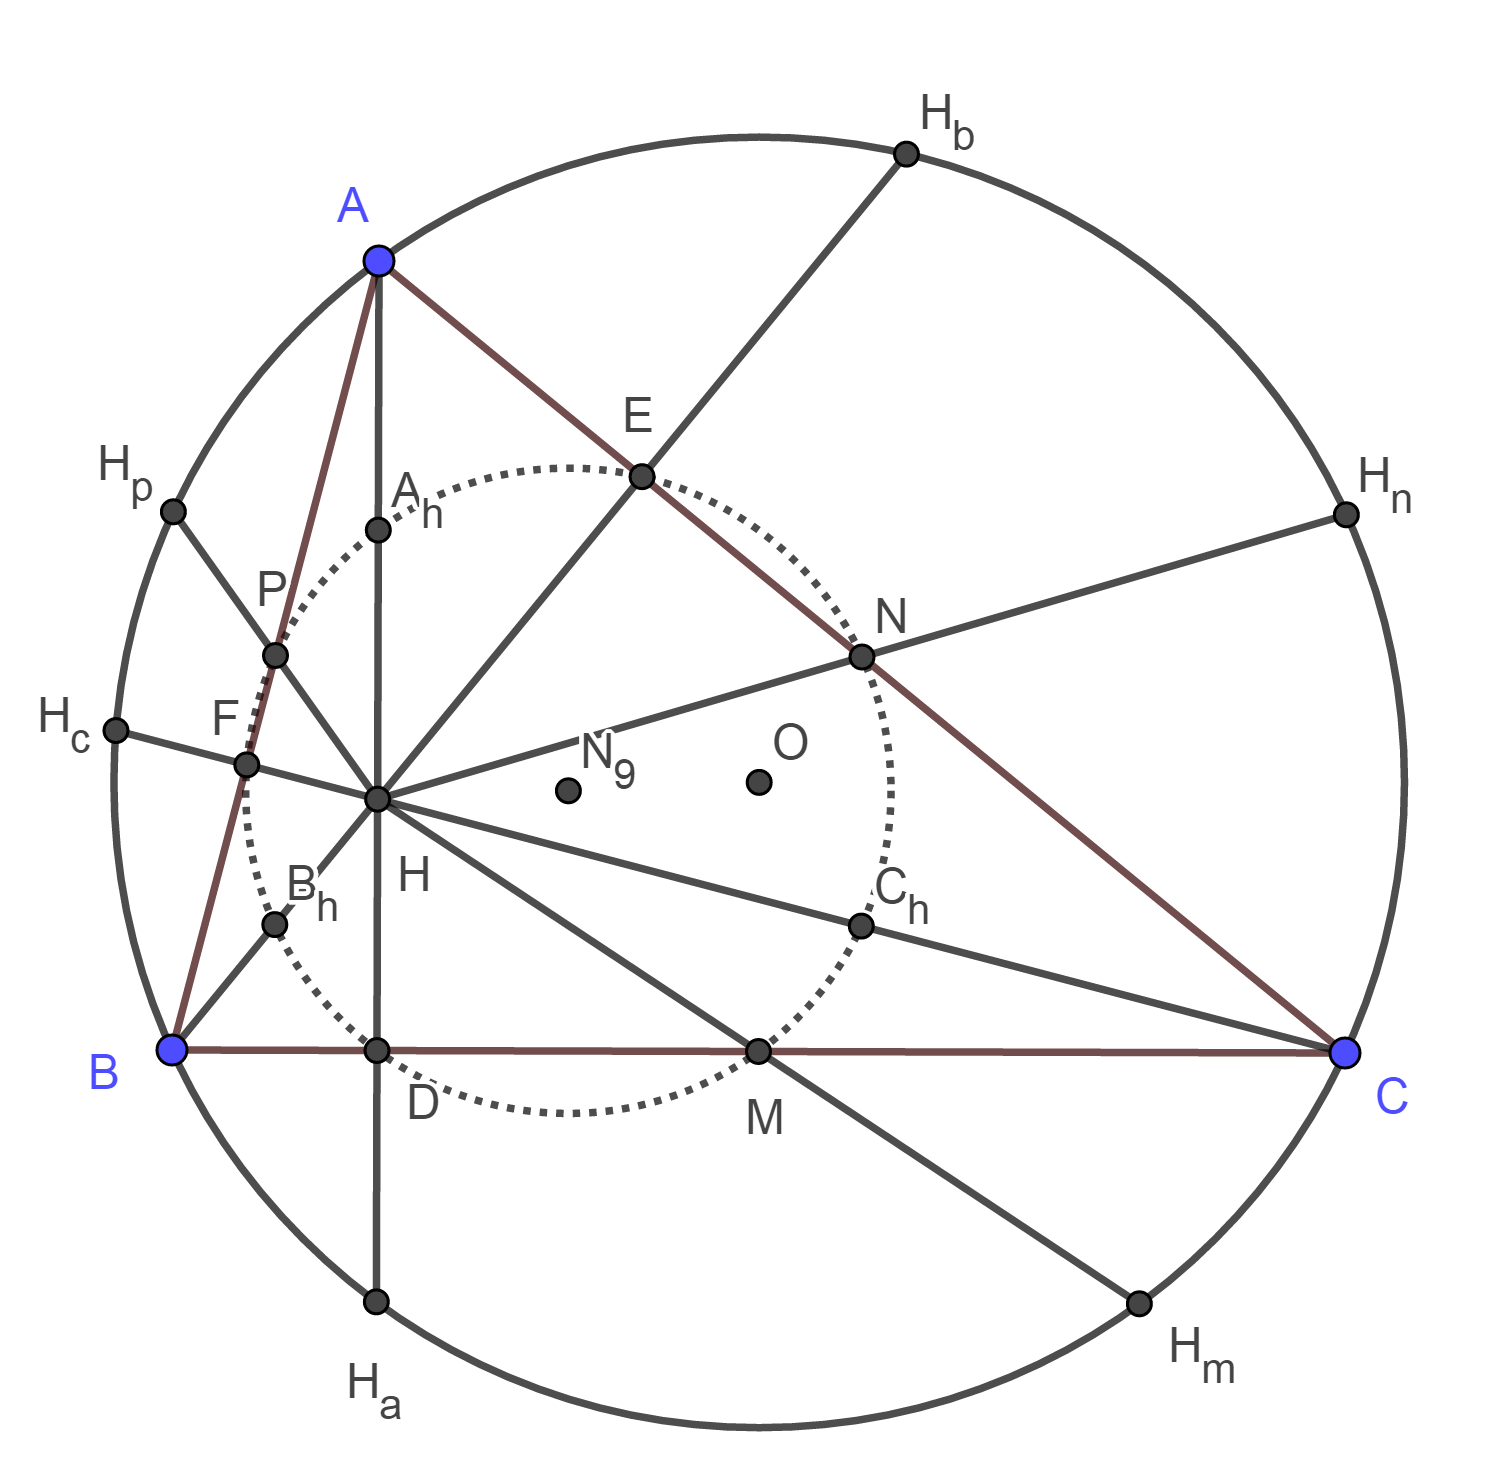
\includegraphics[width=6cm]{fusyta.png}
\end{figure}
Kita bahkan mengetahui titik pusat dan jari-jari $\omega_9$, yaitu $N_9$ titik tengah dari garis $OH$ dan dengan jari-jari setengah dari jari-jari lingkaran luar $\Delta ABC$.

\section{Properti dari $\omega_9$}
Berikut adalah beberapa properti yang berhubungan dengan lingkaran sembilan titik $\omega_9$ :
\begin{enumerate}
    \item $A_hM, B_hN, C_hP$ adalah diameter dari $\omega_9$.
    \item $OA_h$ sejajar dengan $MH$; $OB_h$ sejajar dengan $NH$; $OC_h$ sejajar dengan $PH$.
    \item Untuk sebarang titik $X$ di lingkaran luar $\Delta ABC$ dan jika $Y$ adalah perpotongan ruas garis $HX$ dengan $\omega_9$, maka $HY = YX$
    \item Titik berat $\Delta ABC$, $G$, segaris dengan $O, N_9, $ dan $H$. Selain itu, $HN_9:N_9G:GO = 3:1:2$. Garis yang memuat keempat titik ini biasa disebut juga sebagai \textbf{Garis Euler} dari segitiga $ABC$.
    \item Jika $O_a,O_b,O_c$ berturut-turut adalah titik pusat lingkaran singgung $\Delta ABC$ yang berseberangan dengan $A,B,C$, maka lingkaran sembilan titik dari segitiga $O_aO_bO_c$ adalah lingkaran luar dari segitiga $ABC$.
\end{enumerate}
% Petunjuk untuk bukti : \begin{enumerate}
%     \item Tinjau bahwa $\angle{A_hDM} = \angle{B_hEN} = \angle{C_hFP} = 90^\circ$.
%     \item Karena $A_hM$ diameter, maka $A_hN_9 = N_9M$. Tinjau bahwa $OM$ sejajar dengan $A_hH$. Tinjau pula bahwa $ON_9 = N_9H$. Maka, $A_hHMO$ adalah jajargenjang dan konsekuensinya, $OA_h$ sejajar dengan $MH$.
%     \item Tinjau bahwa $\omega_9$ adalah homotethy dari lingakaran luar $ABC$ dengan pusat $H$ dan skala $\frac{1}{2}$.
%     \item Tinjau bahwa $G$ adalah titik yang terletak di segmen garis $AM$ dengan rasio $AG:GM = 2:1$. Tinjau pula bahwa $AH = 2AA_h = 2OM$. Maka $G$ terletak di garis $OH$ dengan rasio $HG:GO = 2:1$.
%     \item Misalkan $I$ adalah titik pusat lingkaran dalam $\Delta ABC$. Karena $O_a$ adalah perpotongan garis bagi luar sudut $B$ dan $C$, maka $\angle{IBO_a} = \angle{ICO_a} = 90^\circ$. Akibatnya, $I$ adalah titik tinggi $\Delta O_aO_bO_c$ dengan $A,B,C$ sebagai kaki tingginya.
% \end{enumerate}

\end{document}
